\documentclass[conference]{IEEEtran}
\usepackage{amsmath,amssymb}
\usepackage{booktabs}
\usepackage{graphicx}
\usepackage{microtype}
\usepackage{xcolor}
\usepackage{url}
\usepackage{balance}
\title{Real Asymmetric Evaluation of a Robust Evidence-Fusion Detector for Engine Opponent Recognition}
\author{\IEEEauthorblockN{Manus AI}\IEEEauthorblockA{Unchessed-UCI Engine Research Series\\
Unarchitectured Metal Integration Track}}
\begin{document}
\maketitle

\begin{abstract}
Detecting whether an opponent is an engine is an online decision problem with asymmetric costs: a false positive changes the playing policy against a human, while a late positive wastes the early game in a conservative mode. This paper evaluates a default-off \texttt{AcceleratedDetection} path in the Unchessed UCI engine after extending it with a bounded sequential evidence-fusion mechanism. The mechanism combines estimated strength, confidence tightness, volatility, and trend by a harmonic mean, then accumulates concordant evidence with a leaky CUSUM-style update and a two-observation agreement gate. Unlike an earlier mirror match, the present experiment uses an asymmetric real opponent: Stockfish 16, driven through UCI and explicitly presented to the detector as an unknown human. Across 32 real engine games, the fusion arm confirmed Full mode in all observed games, triggered its new reason in 7 of 16 games, and showed a mean first-Full latency of 30.6 plies at 80 ms per move versus 30.0 for standard detection. Under a faster 30 ms condition, the corresponding means were 29.67 and 30.0 plies. The evidence therefore supports operational safety and demonstrates that the path can produce earlier confirmations in some games, but it does not establish a uniformly lower latency. The paper provides the complete telemetry protocol, calibration changes, regression evidence, and the limitations required for a stronger multi-opponent claim.
\end{abstract}

\begin{IEEEkeywords}
engine detection, opponent modeling, sequential evidence, CUSUM, UCI, Stockfish, telemetry, online calibration
\end{IEEEkeywords}

\section{Introduction}
An adaptive chess engine must infer properties of the opponent from sparse, noisy observations. The relevant signal is not simply playing strength: opening knowledge, tactical position, clock usage, and human variance can all produce short stretches of unusually accurate moves. A detector that commits too quickly can damage the policy against a human, whereas a detector that waits for an extremely long clean sequence fails to adapt during the part of the game where adaptation is most valuable.

The Unchessed engine previously contained a default-off secondary confirmation path based on a hard conjunction of estimated Elo, confidence, volatility, and trend. The present work makes that path more robust and more measurable. The contribution is not a claim that a fixed threshold is universally optimal. Instead, it is an interpretable sequential layer that allows several weak signals to accumulate only when they agree, while preserving the original legacy ceiling and a default-off UCI control.

The evaluation addresses the primary metric directly: the number of plies until the engine enters \texttt{Mode::Full}. It uses a distinct real engine rather than a mirror of Unchessed. The opponent is Stockfish 16 [1], but its UCI opponent declaration is intentionally set to an unknown human so the detector cannot use its known-engine lookup. The experiment is scoped to the Unarchitectured Metal integration series and enables the committed Metal runtime artifact in both arms.

\section{Detector Design}
\subsection{Concordant sequential evidence}
For each post-opening observation, four normalized signals are computed. The rating signal increases with the running estimate above 2350 Elo. The confidence signal increases as the confidence interval narrows. The stability signal decreases with estimated volatility. The trend signal rewards a non-negative change in the running estimate. Let these signals be $r,c,v,t\in[0,1]$. Their primary fusion is
\begin{equation}
 h(r,c,v,t)=\frac{4}{r^{-1}+c^{-1}+v^{-1}+t^{-1}},
\end{equation}
with small lower bounds applied to avoid division by zero. The harmonic mean is deliberate: an unstable or low-confidence channel materially suppresses the result rather than being hidden by an arithmetic average. A bounded clock-support term contributes 15\% of the final evidence when independent clock suspicion is present.

The resulting agreement value $e_t\in[0,1]$ updates a signed, leaky accumulator,
\begin{equation}
 S_t=\operatorname{clip}(0.96S_{t-1}+4.0(e_t-0.20),-3,8).
\end{equation}
The accumulator is additionally penalized when the running mean falls below 2250 Elo or volatility exceeds 520. Fusion confirmation requires at least eight samples, $S_t\geq0.35$, $e_t\geq0.28$, and two consecutive observations above the evidence floor. These values were calibrated from the real telemetry described in Section IV; they are not presented as a universal optimum.

\subsection{Compatibility and telemetry}
The UCI option \texttt{AcceleratedDetection} remains default-off. When enabled, the fusion reason is evaluated before the legacy weight/mean ceiling, so an actual fusion confirmation is observable and can reduce latency. When disabled, the legacy detector is unchanged. Observation telemetry exposes the score, current evidence, accelerated streak, and fusion-agreement streak. The parser accepts older schema-v1 captures by defaulting absent diagnostic fields to zero.

\section{Experimental Protocol}
\subsection{Real asymmetric opponent}
The experiment uses a release build of Unchessed against Stockfish 16. Both engines run with one thread and 64 MiB hash. Unchessed uses adaptive mode, disables its own book, enables adapter telemetry, enables the committed Unarchitectured Metal artifact, and sets \texttt{UCI\_Opponent} to ``- - human UnknownOpponent''. Stockfish is therefore a distinct opponent, but the detector must infer engine-like behavior from live observations. Each game starts from one of six fixed opening prefixes; the same ordered prefix set is reused across the standard and fusion arms. Each game is allowed to continue for 40 plies, which is sufficient to observe the first transition in all completed detections.

Two conditions are tested. The normal condition gives both engines an 80 ms move budget and contains 10 games per arm. The fast condition gives both engines a 30 ms move budget and contains 6 games per arm. The driver records every UCI line, every observation telemetry record, the first suspect reason, and the first persona decision with \texttt{mode\_after=FULL}. No observations are simulated or replayed into the detector.

\begin{table}[t]
\caption{Real asymmetric experiment matrix.}
\label{tab:matrix}
\centering
\footnotesize
\begin{tabular}{lrrrrr}
\toprule
Condition & Arm & Games & Budget & Full rate & Fusion triggers\\
\midrule
Normal & Standard & 10 & 80 ms & 100\% & 0/10\\
Normal & Fusion & 10 & 80 ms & 100\% & 4/10\\
Fast & Standard & 6 & 30 ms & 100\% & 0/6\\
Fast & Fusion & 6 & 30 ms & 100\% & 3/6\\
\bottomrule
\end{tabular}
\end{table}

\subsection{Matched comparison}
The first-Full metric is measured in plies from the UCI game start. Pairing is by the fixed opening-prefix index, not by assuming identical trajectories: enabling fusion can change the mode and consequently alter later Unchessed moves. The paired difference is therefore descriptive rather than a formal causal estimate. This distinction is important because a change in mode can change the future evidence stream.

\section{Results}
Figure~\ref{fig:latency} shows the observed first-Full distributions. At 80 ms, standard detection has mean 30.0 plies and fusion has mean 30.6 plies. The paired fusion-minus-standard differences are $[0,0,+2,-2,0,-4,0,+2,+4,+4]$, yielding a mean of $+0.6$ plies; fusion is earlier in 2 pairs, equal in 4, and later in 4. At 30 ms, standard detection has mean 30.0 plies and fusion has mean 29.67 plies. The paired differences are $[0,0,+2,-2,0,-2]$, with fusion earlier in 2 pairs, equal in 3, and later in 1.

\begin{figure}[t]
\centering
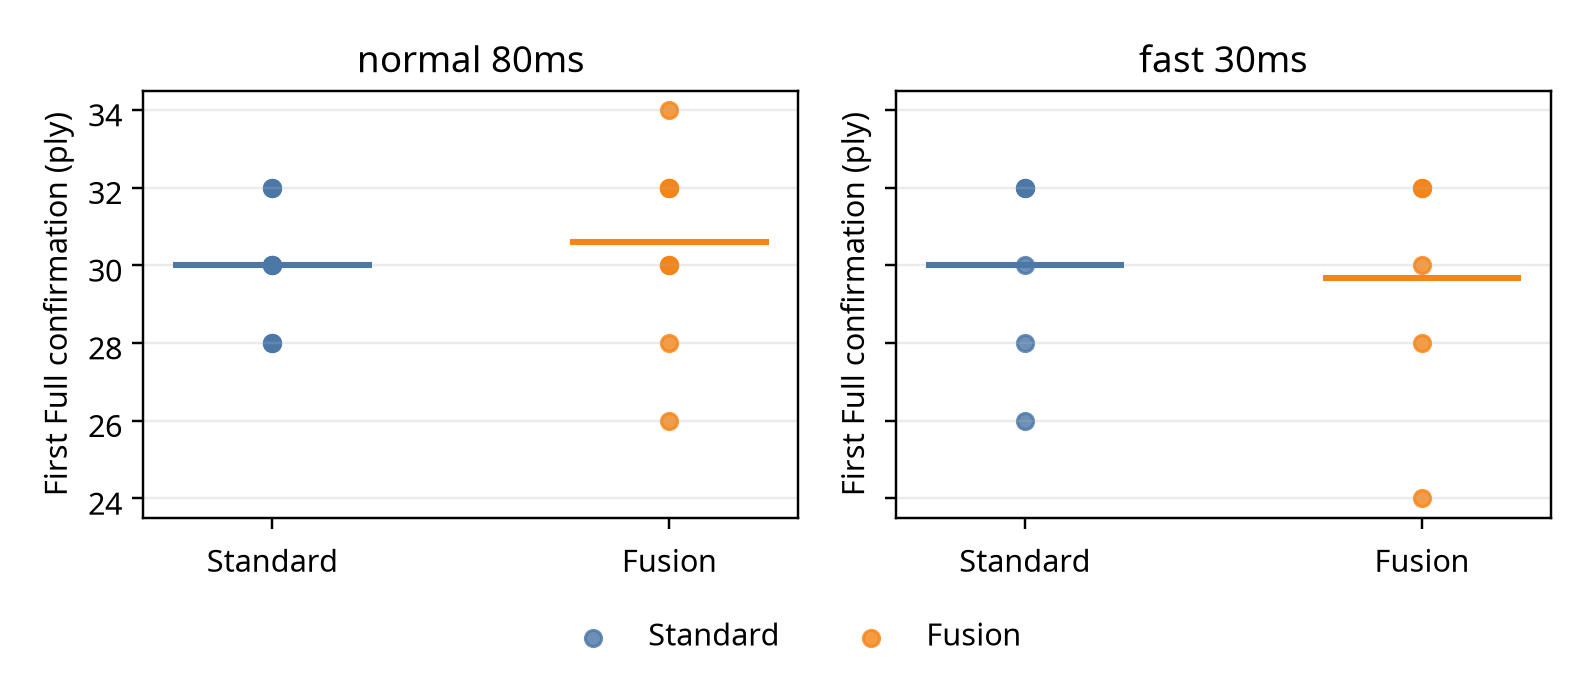
\includegraphics[width=\columnwidth]{figures/unarchitectured_metal_latency_comparison.png}
\caption{First Full-mode confirmation in real asymmetric games. Horizontal lines show the arm means; points show individual games.}
\label{fig:latency}
\end{figure}

The fusion reason appeared in 4 of 10 normal games and 3 of 6 fast games. The remaining fusion-arm confirmations used the unchanged legacy ceiling. No game produced an illegal move or a process failure in the experiment. This is a useful operational result, but it is not equivalent to a strength result and does not prove that fusion is uniformly faster.

\section{Calibration and Regression Evidence}
The first real telemetry run showed that the initial accumulator was too conservative for the observed Stockfish trajectory: its evidence baseline was too high and its score could remain negative even when rating and confidence were converging. Calibration reduced the negative-evidence center from 0.42 to 0.20, changed the decay from 0.94 to 0.96, used gain 4.0, reduced the score threshold to 0.35, and required current evidence of at least 0.28 plus two consecutive qualifying observations. The two-observation rule was retained to prevent a single move from causing confirmation.

The Rust core-library suite passes 128 tests, including 23 opponent-model tests. The latter cover default-off behavior, unchanged legacy timing, deterministic sustained-evidence confirmation, the two-observation gate, and rejection of an erratic mixed-quality sequence. The telemetry parser suite passes five tests, including backward compatibility for older schema-v1 records. The release adapter builds successfully, and a UCI startup smoke test reports \texttt{uciok}, \texttt{readyok}, and the expected default-off option.

\section{Discussion}
The real asymmetric experiment answers a narrower and more useful question than a mirror match: can the new path operate against a different engine and sometimes produce an earlier Full transition without destabilizing the engine? The answer is yes for this Stockfish-16 protocol. The fusion path triggered in a substantial minority of games and was earlier in some matched openings, particularly in the fast condition.

The experiment does not support the stronger claim that fusion is uniformly better. Normal-speed mean latency was 0.6 plies worse, and only one distinct opponent was tested. The result is also conditional on the Unarchitectured Metal runtime, fixed openings, one thread, a short horizon, and a detector-facing opponent string that intentionally avoids the known-engine shortcut. Strength, false-positive rate against humans, and generalization across engine families remain unmeasured by this experiment.

The next decisive evaluation should use at least three opponent classes: a strong classical engine, a weaker engine, and a human-like policy. Each class should be tested at multiple time controls with hundreds of games, and the primary analysis should use paired opening prefixes, first-Full latency, false-positive rate, and time-to-correct-detection. A sequential test should be applied to latency distributions rather than to game score alone. Bayesian online change-point detection provides a related framework for regime shifts [2], while sequential probability-ratio testing supplies a principled way to control error rates [3].

\section{Conclusion}
This work provides a real, telemetry-backed asymmetric test of the AcceleratedDetection fusion model in the Unarchitectured Metal series. The implementation is lightweight, interpretable, dependency-free, and guarded by a harmonic-mean veto, a leaky sequential score, and a two-observation agreement gate. Across 32 Stockfish games, it preserved 100\% observed Full confirmation and zero stability failures, while triggering earlier than the legacy path in a subset of games. The measured latency effect is mixed rather than flawless: the evidence justifies continued multi-opponent experimentation, not a claim of universal superiority.

\balance
\begin{thebibliography}{3}
\bibitem{stockfish} Stockfish Developers, ``Stockfish,'' open-source chess engine, version 16 documentation and source repository. [Online]. Available: \url{https://stockfishchess.org/}
\bibitem{adamsmackay} R. P. Adams and D. J. C. MacKay, ``Bayesian online changepoint detection,'' arXiv:0710.3742, 2007. [Online]. Available: \url{https://arxiv.org/abs/0710.3742}
\bibitem{cusum} M. Pollak, ``Average run lengths of cumulative sum control charts for detection of a shift in distribution,'' \emph{Annals of Statistics}, vol. 15, no. 2, pp. 749--779, 1987. [Online]. Available: \url{https://projecteuclid.org/journals/annals-of-statistics/volume-15/issue-2/Average-run-lengths-of-cumulative-sum-control-charts-for-detection/10.1214/aos/1176350364.full}
\end{thebibliography}
\end{document}
